\documentclass[a4paper]{article}

\usepackage{graphicx} 
\usepackage[english]{babel}
\usepackage{graphicx}
\usepackage{float}
\usepackage{logicproof}
\usepackage{amssymb}
\usepackage[a4paper,top=3cm,bottom=2cm,left=2cm,right=2cm,marginparwidth=1.75cm]{geometry}

\begin{document}

\begin{titlepage}
    \newcommand{\HRule}{\rule{\linewidth}{0.5mm}}
    \center

    \textsc{\LARGE Delft University of Technology}\\[1cm]

    \textsc{\Large Reasoning \& Logic}\\[0.2cm]
    \textsc{\large CSE1300}\\[1cm]
    \HRule \\[0.8cm]
    { \huge \bfseries Assignment: TA-check 2}\\[0.7cm]
    \HRule \\[2cm]
    \large
    \emph{Authors:}\\
    Joris Rijs (5880998) \& Sebastiaan Beekman (5885116)\\[1.5cm]
    {\large \today}\\[5cm]
    
\includegraphics[width=0.6\textwidth]{images/TU_delft_logo.jpg}\\[1cm]
    \vfill
\end{titlepage}

\newpage
\tableofcontents

\newpage
\section{Question 1}

For each of the following statements, indicate whether they are \textit{necessary} for $8 | n$ with \textit{n} an arbitrary integer. Give a convincing argument for your answer.
\begin{itemize}
    \item $ n > 3  $ \\
    Yes this attribute is necessary, however as the given statement works with integers from which we assume that the answer should also be an integer.
    With this in mind, any integer which is smaller than 8 (which also includes the limiter 3) will result in an outcome which is not an integer.
    Knowing this, n should be greater or equal to 8,this will hold as the result of $8 \mid 8 = 1$ which results in a prime factor.
    % No, as one of the prime factors for 8 which where n \s 3 is 2.
    % This is on the basis that 8 is divisible by 2 as well as 2 being a prime number, this makes numbers n smaller than
    \item $ 512 | n^3 $ \\
    Yes this statement will hold however it is not necessary for the original statement, as the given statement can be simplified by taking the cube root of 512.
    This equates to $8 \mid n $, which is equivelant to the original statement.
    \item $ 7 \nmid n $ \\
    No, this statement is not necessary, this does not add anything to the original statement.
    Another argument for the missing necessity is that there are arbitrary \textit{n} values which are both devisable by 8 and 7 at the same time.
    This is on the premise that any arbitrary integer is allowed to be chosen for \textit{n} .
\end{itemize} 

For each of the following statements, indicate whether they are \textit{sufficient} for $5 | n$.
As a general simplification, the base statement can be rewritten as \textit{n = 5 * k} which states that any number divisable by 5 is any number which is a multiple of 5.

\begin{itemize}
    \item $ 5  \sqrt[2]{n} $ \\
    The given statement is not valid. if we use the simplification given it is not possible to get a multiplication which results in the result of 
    The only way to get the square root of 5 is to multiply 5 to the power 1/2, this will mathematically result in the same answer as square root of 5.
    \item $ 3 \nmid n $ \\
    To start, we can simplify the formula to n  3 * k where k is any arbitrary integer.
    On this basis we can say that the statement is not sufficient as that there are integers which are a multiple of 5 / are devisable by 5 which are also a multiple of 3 / devisable by 3.
    This makes the statement false thus not sufficient.
    \item $ n = 25^k (k \ge 3) $ \\ 
    The given statement is sufficient on the basis that $(25^k)$ is equivelant to $ ((5^2)^k) $ which is equivelant to $ (5^{2k}) $.
    This means that the base integer is 5 and thus the product of the given statement is devisable by 5 thus making both statements true, making the given statement sufficient.
    
\end{itemize}

<<<<<<< HEAD
\newpage
\section{Question 2 - Tarski's World}
\subsection{(a)}
In Tarski's world, it is possible to describe situations using formulas whose truth can be evaluated,
which are expressed in a first-order language that uses predicates such as Rightof(x,y),
which means that x is situated—somewhere, not necessarily directly—to the right of y, or Blue(x), which means that x is blue.
In the world in Figure 2.9 in Delftse Foundations of Computation (p. 30), for instance,
the formula$\forall $x(Triangle(x) $\rightarrow $ Blue(x)) holds, since all triangles are blue, but the converse of this
formula, $\forall $x(Blue(x) $\rightarrow $ Triangle(x)), does not hold, since object c is blue but not a triangle.

\begin{figure}[H]
    \centering
    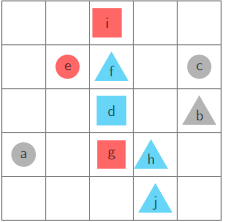
\includegraphics[]{images/tarski-world-example-1.png}
    \caption{An instance of a Tarski World.}
    \label{fig:Tarski}
\end{figure}
\ \\
\textbf{Alfred Tarski} contributed much to the semantics of first-order languages and the systematic development of the concept of truth.
In the program Tarski's World, described in the book Language, Proof and Logic by Barwise and Etchemendy,
a 'Tarski World' is a visualization of a 'mathematical structure,' a core concept in that theory: a structure is a description of a 'situation' wherein one can
evaluate whether a statement in a given first-order language (say, T) is true or false. A structure
contains a domain with objects, plus an indication of all (combinations of) objects with the properties
denoted by the predicate symbols in the language T: Blue(a) is true in a structure (e.g. named A) in
which the object with the name 'a' belongs to the set of objects with the property of being blue. That
set is called $B^A$: the set in structure A that indicates which objects have the property indicated by
predicate symbol B. In Tarski's World, color indicates to which set each object belongs, which could
be notated more generally by describing the set B as $B^A$ = \{a,c,e,g\}. The relation that corresponds
to the predicate RightOf is indicated by the positioning between the objects, but this can be denoted
more generally by describing the relation as the set (see chapter 1) of all pairs (x,y) $\in $ D x D for
which x is situated right of y in the picture: $RightOf^A$ = \{(b,a), (c,a), (d,a), (c,f),...\}.
\subsubsection{(I)}
Give the structure that is visualized in Figure 1 (of this document) in the abstract way
as described above. Take another good look at section 2.4.4 in the book, where you can find
explanations about what this should entail. You may leave out LeftOf, AboveOf, and BelowOf.
\\\\
D = \{a,b,c,d,e,f,g,h,i,j\}\\
$Blue^A$ = \{d,f,h,j\}\\
$Red^A$ = \{e,g,i\}\\
$Grey^A$ = \{a,b,c\}\\
$Square^A$ = \{d,g,i\}\\
$Circle^A$ = \{a,c,e\}\\
$Triangle^A$ = \{b,f,h,j\}\\
$RightOf^A$ = \{(b,a), (c,a), (d,a), (e,a), (f,a), (g,a), (h,a), (i,a), (j,a), (b,e), (c,e), (d,e), (f,e), (g,e), (h,e), (i,e), (j,e), (b,i), (c,i), (h,i), (j,i), (b,f), (c,f), (h,f), (j,f), (b,d), (c,d), (h,d), (j,d), (b,g), (c,g), (h,g), (j,g), (b,h), (c,h), (b,j), (c,j)\}
\subsubsection{(II)}
D = \{a,b\}\\
$Blue^B$ = \{a\}\\
$Grey^B$ = \{b\}\\
$Square^B$ = \{b\}\\
$Triangle^B$ = \{a\}
\\\\
Arguments:
\begin{itemize}
    \item $\exists $x(Triangle(x) $\vee $ Blue(x)), see a
    \item $\exists $x(Square(x) $\wedge $ Grey(x)), see b
    \item $\forall $y(Circle(y) $\rightarrow $ Red(y)), no circles
    \item $\forall $z(Triangle(x) $\rightarrow $ $\neg $Grey(z)), see a
\end{itemize}
\subsubsection{(III)}
A counter example is a Tarski World with a single entity. An entity can never be left or right of itself, so in the claim $\forall $x$\forall $y(RightOf(x,y) $\leftrightarrow $ LeftOf(x,y)) one side is always false and the other is always true (due to the not). This means that the claim is false.

=======
>>>>>>> 8efc47d314599baa47b2e24a17998231cdcba535
\newpage
\subsection{(b)}
For the following invalid arguments, give suitable counterexamples. A counterexample is a structure
as in question 'a', in which all premises (if any) hold, while the conclusion does not hold. You also
need to specify which sets in your structure correspond to which predicate symbols in the formulas.
Note that the domain of a structure cannot be empty. Each time, explain why your structure forms
a counterexample.
\\\\
As an example consider the following argument:\\
$\exists $x(P(x) $\wedge $ Q(x)), $\forall $x(Q(x) $\rightarrow $ R(x)) $\therefore $ $\forall $x(P(x) $\rightarrow $ R(x))
\\\\
What's being claimed is that if there is an object with property P that it also has property Q, and
all objects that have Q also have R, then all all objects with P have R as well. This is clearly not
the case, as is shown by the following structure C with domain D = \{4, 5\}. Let $P^c$ = \{4, 5\} and
$Q^c$ = $R^c$ = \{4\}. Now the first premise holds (take x = 4), the second one holds as $Q^c$ = $R^c$, but
the conclusion does not hold: take x = 5.\\
\subsubsection{(I). $\exists $x(P(x)) $\therefore $ $\forall $x(P(x))}
Structure A with domain D = \{a,b\}\\
Let $P^A$ = \{a\}\\
The first premise holds, but the conclusion does not: take x = b.
\subsubsection{(II). $\therefore $ $\forall $xQ(x)}
Structure B with domain D = \{a\}\\
The (non-existent) premises hold, but the conclusion does not because it is not a tautology.

\subsubsection{(III). $\forall $x(P(x,x)) $\therefore $ $\forall $x$\forall $y(P(x,y))}
Structure C with domain D = \{a,b\}\\
Let $P^C$ = \{(a, a),(b, b)\}\\
The first premise holds, but the conclusion does not: take x = a \& y = b.
\subsubsection{(IV). $\neg $$\forall $x(P(x) $\wedge $ $\exists $y($\neg $Q(x,y))), $\forall $x($\neg $P(x) $\rightarrow $ $\exists $y(Q(x,y))) $\therefore $ $\forall $x$\exists $y(Q(x,y))}
Structure D with domain D = \{a,b\}\\
For the first premise, let $P^D$ = \{b\} and $Q^D$ = \{(a,a),(a,b)\}.\\
For the second premise, let $P^D$ = \{b\} and $Q^D$ = \{(a, a)\}.\\
The premises hold, but the conclusion does not: (a, a), (b, ?)

\subsubsection{(V). $\neg $$\forall $x(P(x) $\rightarrow $ $\exists $yQ(x,y)), $\forall $x$\forall $y(R(x,y) $\rightarrow $ (P(y) $\vee $ Q(x,y))) $\therefore $ $\exists $z($\neg $P(z) $\vee $ $\forall $y(Q(z,y) $\wedge $ $\neg $R(y,z)))}
Structure E with domain D = \{a,b,c\}\\
For the first premise, let $P^E$ = \{a,b,c\} and $Q^E$ = \{\}.\\
For the second premise, let $R^E$ = \{(a,a),(a,b),(a,c)\} $P^E$ = \{a,b,c\}, $Q^E$ = \{(a,a),(b,a),(c,a)\}.\\
The premises hold, but the conclusion does not: take z = a \& y = b.

\newpage
\section{Question 3}
For each of the following abstractly formulated claims, outline a proof for the claim. Highlight what proof techniques you would use in your proof. For example for : $ \forall x \ (P(x) \to Q(x))$, we would answer: Take an arbitrary x such that \textit(P(x)) holds. Now we show that \textit{R(x)} holds. Since x was arbitrarily chosen, it will hold for all x.\\

\textbf{a} $ \exists x \ (P(X))$\\ 
The given statement can be proven by existence.
This can be done by finding a value of x which holds, for example: there is an even prime number.
This can be formally written as:
{
    \noindent
    \setlength\subproofhorizspace{2em}
    \begin{logicproof}{1}
        \exists x \ (P(X)) & premise \\
        \exists x \ (P(X)) & premise \\\hspace*{-30pt}
        \textbf{True} & \textbf{conclusion} 
    \end{logicproof}
}

\textbf{b} $ \forall x \ (P(x) \iff Q(x))$\\
The given statement can be proven by using both generalization and contrapositive.
To start, the given statement can be simplified to $ \forall x \,((P(x) \to Q(x)) ^ (Q(x) \to P(x)))$.
This allows for the ability to proof the first and second statement separately.
we need to choose an arbitrary x for which \textit{P(x)} holds.
{
    \noindent
    \setlength\subproofhorizspace{2em}
    \begin{logicproof}{1}
        \forall x \, (P(x) \to Q(x)) & premise \\
        \forall x \, P(x) & premise \\\hspace*{-30pt}
        \forall x \, Q(x) & \textbf{conclusion} 
    \end{logicproof}
}
{
    \noindent
    \setlength\subproofhorizspace{2em}
    \begin{logicproof}{1}
        \forall x \, (Q(x) \to P(x)) & premise \\
        \forall x \, P(x) & premise \\\hspace*{-30pt}
        \forall x \, \neg Q(x) & \textbf{conclusion} 
    \end{logicproof}
}

\textbf{c}  $\forall x \ (\neg P(x) \to \neg Q(x))$\\
The given statement can be proven doing a proof by generalization.
First, the given statement can be rewritten to $ \forall x \, P(x) \vee \neg Q(x))$.
If we use an arbitrary value for x for which \textit{P(x)} holds, then the statement will hold as only one of the statements needs to be true for the proof to be valid.
This can formally be written as
{
    \noindent
    \setlength\subproofhorizspace{2em}
    \begin{logicproof}{1}
        \forall \forall x \, P(x) \vee \neg Q(x)) & premise \\
        \forall x \, P(x) & premise \\\hspace*{-30pt}
        \forall x \, \neg Q(x) & \textbf{conclusion} 
    \end{logicproof}
}

\textbf{d} $ \forall x \ (P(X) \to \exists y \ (R(x,y)))$  \\
The given statement can be proven by generalization and existence.
The structure of the statement is such that x is allowed to be any arbitrary variable $(\forall x)$.
Based on this we can mainly use a proof by existence by finding a y value for which $\exists y \,R(x, y)$ holds.
And as x is allowed to be any arbitrary value, the statement will be true. 
(This should also still be valid if the statement is rewritten to $\forall x \, \neg P(x) \vee \exists y \, (R(x,y))$ as when the second predicate is true and the first predicate is false due to the 'or' operator).
The statement can formally be written as:
{
    \noindent
    \setlength\subproofhorizspace{2em}
    \begin{logicproof}{1}
        \forall \forall x \, \neg P(x) \vee \exists y \, (R(x,y)) & premise \\
        \forall y \, R(x,y) & premise \\\hspace*{-30pt}
        \textbf{True} & \textbf{conclusion} 
    \end{logicproof}
}

\newpage
\section{Question 4}
In the previous homework assignment we saw the disjunctive normal form that every formula can be
rewritten to. Every formula from propositional calculus can also be written as a conjunction of disjunctions,
in conjunctive normal form (CNF). So the formula (p $\vee $ q) is already in conjunctive normal form as the
conjunction of one disjunction, but ((p $\wedge $ q) $\vee $ r) is not in CNF because it is not a conjunction of
disjunctions; rewriting it to ((p $\vee $ r) $\wedge $ (q $\vee $ r)) gives a conjunctive normal form of this formula.
Now rewrite each of the following formulas to an equivalent form in conjunctive normal form. You need
to be able to justify every step you take, so write down every step explicitly. Also make truth tables for
the formulas labeled with '*' to show that the formula in CNF that you have found is equivalent to the
formula in the assignment that you started with.
\subsection{(a). ((a $\wedge $ b) $\rightarrow $ c)*}
($\neg $(a $\wedge $ b) $\vee $ c)\\
($\neg $a $\vee $ $\neg $b $\vee $ c)
\begin{displaymath}
    \begin{array}{|c c c|c|c|}
        a & b & c & ((a \wedge b) \rightarrow c) & (\neg a \vee \neg b \vee c) \\
        \hline
        0 & 0 & 0 & 1                            & 1                           \\
        0 & 0 & 1 & 1                            & 1                           \\
        0 & 1 & 0 & 0                            & 0                           \\
        0 & 1 & 1 & 1                            & 1                           \\
        \hline
        1 & 0 & 0 & 1                            & 1                           \\
        1 & 0 & 1 & 1                            & 1                           \\
        1 & 1 & 0 & 1                            & 1                           \\
        1 & 1 & 1 & 1                            & 1                           \\
    \end{array}
\end{displaymath}
\subsection{(b). $\neg $(a $\rightarrow $ (b $\wedge $ c))*}
$\neg $($\neg $a $\vee $ (b $\wedge $ c))\\
a $\wedge $ $\neg $(b $\wedge $ c)\\
a $\wedge $ ($\neg $b $\vee $ $\neg $c)
\begin{displaymath}
    \begin{array}{|c c c|c|c|}
        a & b & c & \neg (a \rightarrow (b \wedge c)) & a \wedge (\neg b \vee \neg c) \\
        \hline
        0 & 0 & 0 & 0                            & 0                           \\
        0 & 0 & 1 & 0                            & 0                           \\
        0 & 1 & 0 & 0                            & 0                           \\
        0 & 1 & 1 & 0                            & 0                           \\
        \hline
        1 & 0 & 0 & 1                            & 1                           \\
        1 & 0 & 1 & 1                            & 1                           \\
        1 & 1 & 0 & 1                            & 1                           \\
        1 & 1 & 1 & 0                            & 0                           \\
    \end{array}
\end{displaymath}
\subsection{(c). ((a $\vee $ b) $\rightarrow $ (c $\vee $ d))}
($\neg $(a $\vee $ b) $\vee $ (c $\vee $ d))\\
($\neg $a $\wedge $ $\neg $b) $\vee $ (c $\vee $ d)\\
($\neg $a $\vee $ c $\vee $ d) $\wedge $ ($\neg $b $\vee $ c $\vee $ d)
\subsection{(d). $\neg $(p $\rightarrow $ $\neg $(q $\vee $ ($\neg $r $\wedge $ s))}
$\neg $($\neg $p $\vee $ $\neg $(q $\vee $ ($\neg $r $\wedge $ s)))\\
p $\wedge $ (q $\vee $ ($\neg $r $\wedge $ s))\\
p $\wedge $ (q $\vee $ $\neg $r) $\wedge $ (q $\vee $ $\neg $s)

\newpage
\section{Question 5}
\subsection{(a)}
\textbf{In your own words, explain the difference between a function and a predicate}\\
This depends on the definition of a function.
When a function is an algorithm, then a function is a formal definition, which uses predicates, of said algorithm.
On the other hand, a function can be a way to express how a predicate interacts with a structure's domain. For example, a domain of discourse is a set, A, and a predicate is a function from A.
\subsection{(b)}
\textbf{Give an example of a vacuously true statement about the real-world}\\

\end{document}